% !TeX encoding = UTF-8

% 载入 SJTUThesis 模版
\documentclass[type=master,openany]{sjtuthesis}
% 选项
%   type=[doctor|master|bachelor],     % 可选(默认:master),论文类型
%   zihao=[-4|5],                      % 可选(默认:-4),正文字号大小
%   lang=[zh|en|de|ja],                % 可选(默认:zh),论文的主要语言
%   review,                            % 可选(默认:关闭),盲审模式
%   [twoside|oneside],                 % 可选(默认:twoside),双页或单页边距模式
%   [openright|openany],               % 可选(默认:openright),奇数页或任意页开始新章
%   math-style=[ISO|TeX],              % 可选 (默认:ISO),数学符号样式

% 论文基本配置,加载宏包等全局配置
% !TEX root = ./main.tex

\sjtusetup{
  %
  %******************************
  % 注意:
  %   1. 配置里面不要出现空行
  %   2. 不需要的配置信息可以删除
  %******************************
  %
  % 信息录入
  %
  info = {%
    %
    % 标题
    %
    zh / title           = {基于静态单赋值中间语言的函数式编译器\\ 验证方法},
    en / title           = {Verification of Functional Compilers Based on Static Single Assignment Intermediate Representation},
    %
    % 标题页标题
    %   可使用“\\”命令手动控制换行
    % 
    % zh / display-title   = {上海交通大学学位论文\\ \LaTeX{} 模板示例文档},
    % en / display-title   = {A Sample Document \\ for \LaTeX-based SJTU Thesis Template},
    %
    % 关键词
    %
    zh / keywords        = {编译器验证, 形式化方法, 静态单赋值, 函数式编译器},
    en / keywords        = {Compiler Verification, Formal Methods, Static Single Assignment, Functional Compilers},
    %
    % 姓名
    %
    zh / author          = {刘思雨},
    en / author          = {Siyu Liu},
    %
    % 指导教师
    %
    zh / supervisor      = {汪宇霆副教授},
    en / supervisor      = {Assoc. Prof. Yuting Wang},
    %
    % 副指导教师
    %
    % assoc-supervisor  = {某某教授},
    % assoc-supervisor* = {Prof. Uom Uom},
    %
    % 学号
    %
    id              = {121033910117},
    %
    % 学位
    %   本科生不需要填写
    %
    zh / degree          = {专业学位硕士},
    en / degree          = {Master of Engineering},
    %
    % 专业
    %
    zh / major           = {计算机技术},
    en / major           = {Computer Technology},
    %
    % 所属院系
    %
    zh / department      = {计算机科学与工程系},
    en / department      = {Department of Computer Science and Engineering},
    %
    % 答辩日期
    %   使用 ISO 格式 (yyyy-mm-dd);默认为当前时间
    %
    % date                 = {2023-05-18},
    %
    % 标题页显示日期
    %   覆盖对应标题页的日期显示,原样输出
    %
    % zh / display-date    = {2023 年 5 月},
    %
    % 资助基金
    %
    % zh / fund  = {
    %                {国家 973 项目 (No. 2025CB000000)},
    %                {国家自然科学基金 (No. 81120250000)},
    %              },
    % en / fund  = {
    %                {National Basic Research Program of China (Grant No. 2025CB000000)},
    %                {National Natural Science Foundation of China (Grant No. 81120250000)},
    %              },
  },
  %
  % 风格设置
  %
  style = {%
    %
    % 论文标题页 logo 颜色 (red/blue/black)
    %
    % title-logo-color = black,
  },
  %
  % 名称设置
  %
  name = {
    % bib             = {References},
    % ack             = {谢\hspace{\ccwd}辞},
    % achv            = {攻读学位期间完成的论文},
  },
}

% 使用 BibLaTeX 处理参考文献
%   biblatex-gb7714-2015 常用选项
%     gbnamefmt=lowercase     姓名大小写由输入信息确定
%     gbpub=false             禁用出版信息缺失处理
\usepackage[backend=biber,style=gb7714-2015]{biblatex}
% 文献表字体
% \renewcommand{\bibfont}{\zihao{5}\fixedlineskip{15.6bp}}
% 文献表条目间的间距
\setlength{\bibitemsep}{0pt}
% 导入参考文献数据库
\addbibresource{refs.bib}

% 脚注格式
\usepackage[perpage,bottom,hang]{footmisc}

% 定义图片文件目录与扩展名
\graphicspath{{figures/}}
\DeclareGraphicsExtensions{.pdf,.eps,.png,.jpg,.jpeg}

% 确定浮动对象的位置,可以使用 [H],强制将浮动对象放到这里(可能效果很差)
% \usepackage{float}

% 固定宽度的表格
% \usepackage{tabularx}

% 使用三线表:toprule,midrule,bottomrule。
\usepackage{booktabs}

% 表格中支持跨行
\usepackage{multirow}

% 表格中数字按小数点对齐
\usepackage{dcolumn}
\newcolumntype{d}[1]{D{.}{.}{#1}}

% 使用长表格
\usepackage{longtable}

% 附带脚注的表格
\usepackage{threeparttable}

% 附带脚注的长表格
\usepackage{threeparttablex}

% 算法环境宏包
\usepackage[ruled,vlined,linesnumbered]{algorithm2e}
% \usepackage{algorithm, algorithmicx, algpseudocode}

% 代码环境宏包
\usepackage{listings}
\usepackage{xcolor}
\definecolor{dkgreen}{rgb}{0,0.6,0}
\definecolor{ltblue}{rgb}{0,0.4,0.4}
\definecolor{dkviolet}{rgb}{0.3,0,0.5}
% lstlisting coq style (inspired from a file of Assia Mahboubi)
\lstdefinelanguage{Coq}{ 
    % Anything betweeen $ becomes LaTeX math mode
    mathescape=true,
    % Comments may or not include Latex commands
    texcl=false, 
    % Vernacular commands
    morekeywords=[1]{Section, Module, End, Require, Import, Export,
        Variable, Variables, Parameter, Parameters, Axiom, Hypothesis,
        Hypotheses, Notation, Local, Tactic, Reserved, Scope, Open, Close,
        Bind, Delimit, Definition, Let, Ltac, Fixpoint, CoFixpoint, Add,
        Morphism, Relation, Implicit, Arguments, Unset, Contextual,
        Strict, Prenex, Implicits, Inductive, CoInductive, Record,
        Structure, Canonical, Coercion, Context, Class, Global, Instance,
        Program, Infix, Theorem, Lemma, Corollary, Proposition, Fact,
        Remark, Example, Proof, Goal, Save, Qed, Defined, Hint, Resolve,
        Rewrite, View, Search, Show, Print, Printing, All, Eval, Check,
        Projections, inside, outside, Def},
    % Gallina
    morekeywords=[2]{forall, exists, exists2, fun, fix, cofix, struct,
        match, with, end, as, in, return, let, if, is, then, else, for, of,
        nosimpl, when},
    % Sorts
    morekeywords=[3]{Type, Prop, Set, true, false, option},
    % Various tactics, some are std Coq subsumed by ssr, for the manual purpose
    morekeywords=[4]{pose, set, move, case, elim, apply, clear, hnf,
        intro, intros, generalize, rename, pattern, after, destruct,
        induction, using, refine, inversion, injection, rewrite, congr,
        unlock, compute, ring, field, fourier, replace, fold, unfold,
        change, cutrewrite, simpl, have, suff, wlog, suffices, without,
        loss, nat_norm, assert, cut, trivial, revert, bool_congr, nat_congr,
        symmetry, transitivity, auto, split, left, right, autorewrite},
    % Terminators
    morekeywords=[5]{by, done, exact, reflexivity, tauto, romega, omega,
        assumption, solve, contradiction, discriminate},
    % Control
    morekeywords=[6]{do, last, first, try, idtac, repeat},
    % Comments delimiters, we do turn this off for the manual
    morecomment=[s]{(*}{*)},
    % Spaces are not displayed as a special character
    showstringspaces=false,
    % String delimiters
    morestring=[b]",
    morestring=[d]’,
    % Size of tabulations
    tabsize=3,
    % Enables ASCII chars 128 to 255
    extendedchars=false,
    % Case sensitivity
    sensitive=true,
    % Automatic breaking of long lines
    xleftmargin       = 1em,
    xrightmargin      = 1em,
    breaklines=false,
    framexleftmargin  = 1em,
    framexrightmargin = 1em,
    keepspaces        = true,
    backgroundcolor   = \color{gray!10},
    % Default style fors listings
    basicstyle=\normalsize,
    % numbers=left,
    % numberstyle=\small\color{gray},
    % Position of captions is bottom
    captionpos=b,
    % flexible columns
    columns=[l]flexible,
    % Style for (listings') identifiers
    identifierstyle={\ttfamily\color{black}},
    % Style for declaration keywords
    keywordstyle=[1]{\ttfamily\color{dkviolet}},
    % Style for gallina keywords
    keywordstyle=[2]{\ttfamily\color{dkgreen}},
    % Style for sorts keywords
    keywordstyle=[3]{\ttfamily\color{ltblue}},
    % Style for tactics keywords
    keywordstyle=[4]{\ttfamily\color{ltblue}},
    % Style for terminators keywords
    keywordstyle=[5]{\ttfamily\color{dkred}},
    %Style for iterators
    %keywordstyle=[6]{\ttfamily\color{dkpink}},
    % Style for strings
    stringstyle=\ttfamily,
    % Style for comments
    commentstyle={\ttfamily\color{dkgreen}},
    %moredelim=**[is][\ttfamily\color{red}]{/&}{&/},
    literate=
    {\\forall}{{\color{dkgreen}{$\forall\;$}}}1
    {\\exists}{{$\exists\;$}}1
    {<-}{{$\leftarrow\;$}}1
    {=>}{{$\Rightarrow\;$}}1
    {==}{{\code{==}\;}}1
    {==>}{{\code{==>}\;}}1
    %    {:>}{{\code{:>}\;}}1
    {->}{{$\rightarrow\;$}}1
    {<->}{{$\leftrightarrow\;$}}1
    {<==}{{$\leq\;$}}1
    {\#}{{$^\star$}}1 
    {\\o}{{$\circ\;$}}1 
    {\@}{{$\cdot$}}1 
    {\/\\}{{$\wedge\;$}}1
    {\\\/}{{$\vee\;$}}1
    {++}{{\code{++}}}1
    {~}{{$\sim$}}1
    {\@\@}{{$@$}}1
    {\\mapsto}{{$\mapsto\;$}}1
    {\\hline}{{\rule{\linewidth}{0.5pt}}}1
    %
}[keywords,comments,strings]
\lstdefinestyle{lstStyleCode}{%
  aboveskip         = \medskipamount,
  belowskip         = \medskipamount,
  basicstyle        = \ttfamily\zihao{6},
  commentstyle      = \slshape\color{black!60},
  stringstyle       = \color{green!40!black!100},
  keywordstyle      = \bfseries\color{blue!50!black},
  extendedchars     = false,
  upquote           = true,
  tabsize           = 2,
  showstringspaces  = false,
  xleftmargin       = 1em,
  xrightmargin      = 1em,
  breaklines        = false,
  framexleftmargin  = 1em,
  framexrightmargin = 1em,
  backgroundcolor   = \color{gray!10},
  columns           = flexible,
  keepspaces        = true,
  texcl             = true,
  mathescape        = true
}
\lstnewenvironment{codeblock}[1][]{%
  \lstset{style=lstStyleCode,#1}}{}
% 将lstlisting的名称修改为中文
\renewcommand\lstlistingname{图}

% 直立体数学符号
\providecommand{\dd}{\mathop{}\!\mathrm{d}}
\providecommand{\ee}{\mathrm{e}}
\providecommand{\ii}{\mathrm{i}}
\providecommand{\jj}{\mathrm{j}}

% 国际单位制宏包
\usepackage{siunitx}

% 定理环境宏包
\usepackage{ntheorem}
% \usepackage{amsthm}

% 绘图宏包
\usepackage{tikz}
\usetikzlibrary{arrows.meta, shapes.geometric, chains, shadows.blur}

% 一些文档中用到的 logo
\usepackage{hologo}
\providecommand{\XeTeX}{\hologo{XeTeX}}
\providecommand{\BibLaTeX}{\textsc{Bib}\LaTeX}

% 借用 ltxdoc 里面的几个命令方便写文档
\DeclareRobustCommand\cs[1]{\texttt{\char`\\#1}}
\providecommand\pkg[1]{{\sffamily#1}}

% hyperref 宏包在最后调用
\usepackage{hyperref}

% E-mail
\providecommand{\email}[1]{\href{mailto:#1}{\urlstyle{tt}\nolinkurl{#1}}}

% \usepackage{amssymb}
\usepackage{graphicx}
\usepackage[misc,geometry]{ifsym}
\usepackage{caption}
\usepackage{subcaption}
\usepackage{amsmath}
\usepackage{multicol}
\usepackage{multirow}
\usepackage{mathtools}
\usepackage{enumitem}
\usepackage{setspace}
\usepackage{fancyhdr}
\usepackage{etoolbox}
\usepackage{bm}
\usepackage{tabularray}

\newcommand\doubleplus{\mathbin{+\mkern-5mu+}}


\begin{document}

%TC:ignore

% 标题页
\maketitle

% 原创性声明及使用授权书
\copyrightpage
% 插入外置原创性声明及使用授权书
% 此时必须在导言区使用 \usepackage{pdfpages}
% \copyrightpage[scans/sample-copyright.pdf]

% 前置部分
\frontmatter

% 摘要
% !TEX root = ../main.tex

\begin{abstract}[zh]
  静态单赋值(Static Single Assignment, SSA)形式的中间语言(Intermediate Representation, IR)
  被现代主流编译器基础设施广泛采用。
  这是因为它能够实现许多基于数据流分析的编译优化,从而显著提高编译器的编译效率。
  现有的函数式编译器一般会将源程序编译为延续传递风格(Continuation Passing Style, CPS),
  以得到明确的控制流。
  函数式语言编译器如果想利用基于数据流分析的丰富优化,就需要将延续传递风格的程序与静态单赋值中间语言连接起来。
  编译器作为重要的系统软件,其正确性也一直是研究者们不断探讨的方向。
  随着形式化方法理论和工具的发展,编译器的形式化验证已经被证明是确保编译过程正确性的有效方法。

  本文研究了如何将关键的函数式语言编译过程与静态单赋值中间语言通过形式化方法联系起来,
  从而在确保编译正确性的情况下使函数式语言的编译器能够充分利用静态单赋值中间语言的优势。
  我们设计了从延续传递风格的函数式程序到静态单赋值中间语言的转换算法,
  并对该转换算法进行了基于模拟技术的形式化验证。
  建立了这样的联系,才能够使经验证的函数式编译器复用基于静态单赋值的程序分析与编译优化,
  从而使高可靠的函数式编译器得到效率提升。
  本文还以代表性的基础函数式编程语言PCF(Programming Computable Functions)为研究对象,
  应用该经验证的编译过程构建出了PCF语言到LLVM中间语言的函数式编译器。
  具体而言,我们首先读入直接风格的PCF源程序,将其转换为延续传递风格,再编译到静态单赋值中间语言。
  我们对这条编译链的正确性进行形式化验证,并将它与LLVM中间语言连接起来。
  该工作为构建经验证的高性能、高可靠函数式编译器提供了基础。
  本文涉及的所有转换算法和定理证明均在Coq定理证明器中实现。
\end{abstract}

\begin{abstract}[en]
  Intermediate Representation (IR) in Static Single Assignment (SSA) form
  has been widely adopted by modern mainstream compiler infrastructures.
  It facilitates numerous compilation optimizations based on data-flow analysis,
  so as to significantly improve the performance of compilers.
  Existing functional compilers often translate source programs into 
  Continuation Passing Style (CPS) to achieve explicit control flow. 
  To harness the improvement provided by optimizations based on data-flow analysis, 
  a functional compiler needs to establish a connection between 
  programs in CPS and the SSA IR. 
  As essential components of system software, correctness of compilers have been the 
  subject of continuous exploration by researchers.
  With the development of the theory and tools for formal methods, 
  the formal verification of compilers has proven to be an effective approach 
  in ensuring their correctness.
  
  This paper investigates how to formally connect the key processes 
  of functional language compilation with SSA intermediate language, 
  enabling functional language compilers to harness the advantages of SSA 
  while ensuring compilation correctness. 
  In this paper, we design a transformation algorithm from CPS functional programs 
  to SSA intermediate language and formally verify this transformation algorithm 
  using simulation methods. Establishing such a connection enables 
  verified functional compilers to leverage SSA-based program analysis 
  and compilation optimizations, thus enhancing the efficiency of 
  highly reliable compilers for functional languages. 
  Furthermore, this paper takes the representative foundational functional 
  programming language, PCF (Programming Computable Functions), 
  as the source language. Applying the verified compilation process, 
  we construct a functional compiler for translating PCF programs to 
  LLVM intermediate language. Specifically, it involves the initial transformation
  of the direct-style PCF source code into CPS, followed by compilation into the SSA. 
  We formally verify the correctness of this compilation chain and connect it to the LLVM IR. 
  It provides the foundation for constructing a verified, high-performance, 
  and highly reliable functional compiler. All the transformation algorithms and 
  proofs of theorem discussed in this paper have been implemented in the Coq theorem prover.
\end{abstract}


% 目录
\tableofcontents
% 插图索引
\listoffigures*
% 表格索引
\listoftables*
% 算法索引
\listofalgorithms*

% 符号对照表
% !TEX root = ../main.tex

\begin{nomenclature*}
\label{chap:symb}

\begin{longtable}{rl}
  $k$  & 延续变量  \\  
  $B$       & 可观察行为    \\
  $\mathcal{T}$  & 编译过程  \\
  $\sim$       & 程序状态之间的不变式    \\
  $M$  & 度量函数  \\
  $S$       & 程序状态    \\
  $\approx$       & 语义保存性质    \\
  $\Downarrow$  & 程序终止  \\
  $\Uparrow$       & 程序发散    \\
  $\rightarrow$  & 小步操作语义的一步转换  \\
  $\xrightarrow{+}$       & 小步操作语义的一步或多步转换    \\
  $\xrightarrow{*}$  & 小步操作语义的零步或一步或多步转换  \\
  $loc\; [x\mapsto v]$ & 把从$x$到$v$的映射添加到$loc$中  \\
  $\mathcal{F}_{proc}$  & CPS转换  \\
  $\mathcal{G}_{proc}$  & CPS到SSA的转换  \\
  $Comp$  & PCF到SSA的转换  \\
\end{longtable}

\end{nomenclature*}


%TC:endignore

% 主体部分
\mainmatter

% 正文内容
% !TEX root = ../main.tex

\chapter{绪论}


\section{引言}

编译器作为关键系统软件之一,其正确性对于计算机系统的安全运行有重要意义。
这是由于编译器可能在转换程序的过程中引入错误,导致目标程序的行为和源程序不一致,
进而使得在源程序端花费大量精力的测试和验证工作在目标程序层级失效。
虽然对于编译器一般会进行密集的测试,错误编译是小概率事件,但是这种偶发性的
由编译器引入的问题,对于安全关键系统而言是需要考虑的。
工业界长期以来对保障编译器正确性这个问题非常重视。例如,按照航空领域的RTCA DO178B/C标准~\cite{brosgol2010178c},
需要按照和机载软件一样的严格要求对待编译器。
对于庞大的编译器,通过测试找到它的错误其实是比较困难的。
编译器随机测试工具Csmith~\cite{csmith2011}已经发现了四百多个编译器错误,可见编译器中隐藏的风险数量之大。

编译器的形式化验证已被证实可以有效保证编译器的正确性,它从数学层面上确保了编译过程的正确性。
一个著名的例子是经过验证的C编译器CompCert~\cite{leroy2009formally},
它将C语言的一个有代表性的重要子集编译到了支持多种处理器架构的汇编代码(包括PowerPC、ARM、X86和RISC-V)。
其编译过程的正确性(即目标汇编程序保存了源C程序的语义)经过了形式化验证,并在Coq定理证明器中实现。

延续传递风格(Continuation-Passing Style, CPS)是一种函数式程序的中间语言(Intermediate Representation, IR),
它明确了函数式程序的控制流,从而为程序基于控制流的分析和优化提供了便利。
延续传递风格的中间语言在函数式程序的编译器中被
广泛采用\cite{belanger-cpp2013,dargaye2009verification,zoe-oopsla2021,zoe-icfp2021,wang-esop2016}。
然而,这也意味着经验证的函数式编译器不能直接得到主流编译器基础设施(例如LLVM和GCC)的支持。
这些主流编译器基础设施采用静态单赋值(Static Single Assignment, SSA)形式的中间语言。 
SSA中间语言在工业编译器中大大流行,因为它可以通过强制让每个变量只能被赋值一次来实现
便捷而准确的数据流分析(Data-Flow Analysis, DFA),进而实现各种基于数据流分析的激进优化。
许多流行的命令式编程语言(例如Rust~\cite{balasubramanian2017system}和Swift~\cite{zhang2012swift})
使用这些编译器基础设施作为其后端,生成性能优越的代码~\cite{lattner2006introduction}。
一些工业级的函数式编译器也开始采用SSA形式的中间语言。例如,SML-New Jersey的
新版本已经将其后端转向了LLVM~\cite{farvardin2020new}。

在本文中,我们研究了如何构建基于SSA中间语言的经验证的函数式语言编译器。
具体而言,我们设计并验证了从CPS到SSA的转换算法,以便在经验证的编译器领域中将
传统基于CPS的函数式编译器与基于SSA中间语言上工作的主流编译器后端连接起来。
尽管研究人员已经探讨了CPS和SSA程序结构之间的对应关系~\cite{appel1998ssa,ssabook},
和相互转换~\cite{farvardin2020new,kelsey1995correspondence},
但如何对转换算法进行形式化验证仍然是待解决的问题。

本文的主要贡献总结如下:

\begin{itemize}
    \item
    我们的主要贡献是设计和验证了从CPS到SSA的转换算法。该转换过程的源语言是代表性的
    函数式语言PCF\cite{plotkin1977lcf},我们首先需要将其转换为CPS形式。
    转换算法的SSA目标语言是LLVM IR的一种简化版本,保留了LLVM IR的基本结构。
    该转换是基于CPS和SSA结构上的对应关系设计的~\cite{appel1998ssa,kelsey1995correspondence}。
    我们为PCF和SSA语言定义了小步操作语义,使用基于模拟的方法证明目标程序实现了
    源程序的语义保存。据我们所知,这是第一个经过验证的从CPS函数式程序到SSA的转换。
    
    \item 
    我们还利用该经验证的编译链构建了PCF语言的编译器原型。它是部分经过形式化验证的,
    为未来构建更复杂更完整的经验证函数式语言编译器打下基础。
    具体而言,我们首先实现并验证了直接风格PCF语言的CPS转换,并将它连接到经验证的CPS到SSA的编译过程。
    然后,我们通过Vellvm提供的抽象语法(Vellvm是一个经过验证的LLVM基础设施~\cite{zakowski2021modular}),
    将SSA中间语言转换为LLVM IR。
    
\end{itemize}

在本章接下来的内容中,我们首先在\ref{sec:background}节介绍必要的相关背景知识,
并在\ref{sec:related}节讨论了领域内与本课题相关的工作。
在第\ref{ch:overview}章中,我们简要介绍了该部分经验证的PCF编译器原型。
我们在第\ref{ch:trans}章中讨论了CPS转换和CPS到SSA的转换算法设计,
并在第\ref{ch:verify}章中对该编译链进行形式化验证。
本文工作在Coq中的实现和评估将在第\ref{ch:implement}章中介绍。
最后,我们在第\ref{ch:summary}章中对本文内容进行总结。

\section{相关背景} \label{sec:background}

在本节中,我们将对该课题的相关背景进行介绍。
本文工作涉及函数式编程、编译器常用中间语言形式以及编译器形式化验证方法等方向。
首先,我们会介绍函数式编程的概念及其特性。
然后,我们将说明CPS形式是如何帮助函数式程序显式地表示控制流的,
并介绍了静态单赋值中间语言的相关特性以及CPS和SSA结构之间的对应关系。
接下来,我们介绍了在经验证的编译器CompCert中提出的基于模拟技术进行编译器验证的框架~\cite{leroy2009formally}。

\subsection{函数式编程}

函数式编程(Functional Programming)是一种通过应用和组合函数来构建程序的编程范式,
以$\lambda$演算($\lambda$-Calculus)作为其数学基础~\cite{church1985calculi}。
传统命令式编程中,计算通过执行程序语句序更新程序状态来实现。
相比之下,函数式编程中程序由包含函数定义和应用的表达式构成,而计算通过对表达式求值来实现。
函数式程序的一大特点是函数可以作为参数传递,或者被其他函数返回,形成所谓的高阶函数~\cite{sussman1998scheme}。
此外,纯粹函数式程序的执行不会引起改变程序状态的副作用。
这些特点使得函数式程序设计语言编写的程序更加简洁、安全和易于验证~\cite{hudak1989conception},
因此在并发编程、系统内存编程等方面获得了成功应用。

在学术界和工业界中,函数式编程的应用日趋广泛。
除了Haskell~\cite{o2008real}等纯函数式语言,OCaml、Erlang、Scala~\cite{cesarini2009erlang, odersky2014unifying}
等语言都对函数式编程有内生的支持,且诸多命令式编程语言如C++和Rust也在积极的引入函数式编程机制。
本文研究的函数式编程语言是学术界有广泛影响力的PCF(Programming Computable Functions)。
由于PCF可以看作是工业用函数式编程语言的核心,本文的研究结果可被推广至其他函数式语言。
关于PCF语言的更多特性将在第\ref{sec:cps}节中详述。

\subsection{延续传递风格与静态单赋值} \label{sec:bg_cpsssa}

函数式程序的形式有很多种,如直接风格(Direct Style)和延续传递风格(CPS)。
图~\ref{cpsdirect}展示了同样含义的函数式程序在这两种不同表示风格下的例子。
CPS的关键特性在于通过延续明确地表示程序的控制流。
CPS中的延续(Continuation)指的是当前执行节点后所有剩余计算的函数,
该函数需要把当前计算得到的结果作为其输入。
具体来说,CPS函数需要将延续作为额外的参数传入,
当运行该函数得到计算结果后,程序通过调用该延续来传递这个值,也就是``返回''该结果。
以图~\ref{fig:cps2}为例,函数$h$在CPS中的延续参数为$k$,在得到最终结果$z$之后,
程序调用$(k\; z)$以返回$z$,并执行$k$所代表的剩余计算。
当调用CPS函数时,调用者需要提供一个延续函数来表示剩余计算,且在CPS中所有中间结果、控制流中的控制点都需要被明确命名。
这些特点导致用户直接用CPS形式编写代码较为困难,但是由于明确表示的控制流利于程序分析和优化,
CPS是函数式语言编译器中常见的中间表示形式。

\begin{figure}
    % \vspace{-0.3cm}
    \centering
    \begin{subfigure}[b]{0.3\textwidth}
        \flushright
    % \small
     \begin{equation}
        \nonumber
        \begin{aligned}
        &  \mathbf{function}\; h(x,y) = \\
        & \quad (x*x)\; +\; (y*y) \\
        \end{aligned}
    \end{equation}
    \caption{Direct Style}
        \label{fig:ori2}
    \end{subfigure}
 %   \hfill
    \begin{subfigure}[b]{0.6\textwidth}
        \flushleft
        % \small
        \begin{equation}
            \nonumber
            \begin{aligned}
            & \mathbf{function}\; h(x,y,k)= \mathbf{let}\; x_1=x*x\; \mathbf{in} \\
            &  \quad   \mathbf{let}\; y_1=y*y\; \mathbf{in}\; (\mathbf{let}\; z=x_1+y_1\; \mathbf{in}\; (k\; z)) \\
            \end{aligned}
        \end{equation}
        \caption{CPS}
        \label{fig:cps2}
    \end{subfigure}
    \caption{直接风格和CPS形式的示例函数式程序}\label{cpsdirect}
  \end{figure}

Plotkin~\cite{plotkin1977lcf}、Danvy和Nielsen\cite{danvy2007one}等人研究了将直接风格的函数式程序转换为CPS程序的方法。
其中Plotkin的方法需要后续进行管理性缩减(Administrative Reduction),以去除冗余的$\lambda$结构。
Felleisen等人提出了另一种方法非组合式的方法,其基于$\lambda$-演算的语义。
Danvy和Nielsen将这两种方法联系起来,可以只通过一步转换完成,不需要在后续过程中进行管理性缩减。

静态单赋值(SSA)是命令式语言编译器中一种广泛使用的中间语言类型。
在SSA中,每个变量只能在一处被赋值,且被使用之前必须已经被赋值。
这种性质很接近函数式语言中的名字绑定(Name Binding)~\cite{ssabook}。
变量被划分为不同的版本,新版本的变量往往使用原名加下标来表示,以使每个定义得到自己的版本。
$\phi$节点($\phi$-nodes)作为特殊的程序语句被插入到基本代码块的开头,
从而按照前驱基本块的名字生成新变量的赋值语句。
这样一来,变量的使用定义链(Use-def Chains)更加清晰,从而使许多编译器优化算法
在SSA中间语言上能够更好地实现,例如常量传播、无用代码消除、寄存器分配等~\cite{ssabook,kelsey1995correspondence}。
作为示例,图~\ref{ssacfg}展示了一个SSA程序的控制流图(Control-Flow Graph)。
其中,基本代码块$b_2$的前驱基本块可以是$b_1$或$b_2$本身。
不同的前驱基本块对变量$y$有不同的赋值,在$b_1$和$b_2$中变量$y$被赋予了不同版本的名称。
基本块$b_2$开头的$\phi$节点将$y_1$和$y_3$作为参数,根据执行时控制流的实际前驱基本块来
选择正确的版本赋值给新的变量$y_2$。

LLVM IR就是一种基于SSA的中间代码。它作为一种高层次的汇编语言,提供了编译系统的中间层,
使得不同语言可以相互连接起来,复用其后端优化~\cite{lattner2006introduction}。
除了LLVM,还有很多编译器是基于SSA的,例如GCC编译器的中间语言GIMPLE~\cite{callanan2007extending}、
面向微软.NET平台的即时编译中间语言CIL(Common Intermediate Language)~\cite{thai2003net}等。

\begin{figure}[htbp]
    \centering
    % \documentclass{article}
% \usepackage{tikz}
% \usetikzlibrary{chains,shadows.blur}

% \begin{document}
\begin{tikzpicture}[auto,
%   node distance = 12mm,
%   start chain = going right,
  box/.style = {draw,rounded corners,blur shadow,fill=white,
        align=center}]
 \small
 \node[box] (b1) at(0,0)    {$v_1 \leftarrow 1$\\ 
                    $z_1 \leftarrow 8$ \\ 
                    $y_1 \leftarrow 4$};      
 \node[box] (b2) at(3,0)    {$y_2 \leftarrow \phi(y_1,y_3)$\\
                    $x_1 \leftarrow 5 + y_2$ \\
                    $y_3 \leftarrow x_1 * z_1$ \\
                    $x_2 \leftarrow x_1 - 1$ \\
                    $\mathbf{if}\; x_2 = 0$};      
 \node[box] (b3) at(6.5,0)    {$w_1 \leftarrow v_1 +y_3$\\ 
                    $\mathbf{return}\; w_1$};  
 \node at(4.0,1.5) {false};
 \node at(4.8,0.3) {true};

 \coordinate (b1n) at ([yshift=-31] b1);
 \coordinate (b2n) at ([yshift=-43] b2);
 \coordinate (b3n) at ([yshift=-25] b3);

 \node at (b1n)  {$b_1$};
 \node at (b2n)  {$b_2$};
 \node at (b3n)  {$b_3$};
 
 \begin{scope}[rounded corners,-latex]
  \path (b2.60) edge[bend right=50] (b2.120)
        (b1) edge (b2) (b2) edge (b3) ;
%   \draw (b3.230) -- ++(0,-0.3) -| ([xshift=-5mm]b2.west) |-
%   ([yshift=3mm]b2.130) -- (b2.130);
 \end{scope}
\end{tikzpicture}
% \end{document}      
    \caption{SSA程序的控制流图示例}\label{ssacfg}
\end{figure}

Appel等人~\cite{appel1998ssa}发现SSA也是一种函数式语言:$\lambda$演算和SSA虽然有不同的形式,
但它们所做的工作其实是相同的。L. Beringer~\cite{ssabook}给出了SSA的函数式表示,
将SSA中的相关术语与函数式编程中的概念联系起来。
例如,函数式语言中的$let$绑定对应着SSA中的赋值、绑定变量的词法作用域对应着SSA中的可支配区域。
$let$绑定与变量定义点之间的对应关系还延续到了程序结构的其他方面。
与命令式语言中的返回地址或函数指针相似,延续指定了当前代码片段求值完成后程序下一步该如何执行。
SSA中的控制流图对应着函数式编程中的函数,虽然顶层延续的参数在控制流图中并不是明确可见的,
但它对应一个命令式调用中用来保存返回地址的地方。
Kelsey~\cite{kelsey1995correspondence}通过将CPS中的$\lambda$进行标注来区分完整过程、跳转、延续,
进而将被这种标注的CPS程序转换为一种SSA程序。然而,Kelsey工作中的CPS和SSA语言与本文中所使用的差距较大。
Kelsey的CPS语言将二元表达式的参数和条件语句中的条件视为表达式,使其更类似于带有延续元素的标准函数式程序。
例如,在Kelsey的工作中,表达式$k; ((x+y)+z)$是允许的,但在我们的工作中,
它必须转换为$\mathbf{letop}; x_0 = x+y; \mathbf{in}; (\mathbf{letop}; x_1 = x_0+z; \mathbf{in}; k; x_1)$。
此外,Kelsey的转换算法选择先合并CPS过程,然后再将其作为整体进行转换。
因此,SSA程序的顶层单元是一整个过程,没有函数调用,这与本文中使用的基于LLVM IR的SSA语言不同。

\subsection{编译器形式化验证} \label{sec:compcertbackend}

我们使用CompCert~\cite{leroy2009formally}基于模拟(Simulation)技术的形式化验证框架来证明转换过程的正确性。
经过形式化验证的C语言子集编译器CompCert是由INRIA的Xavier Leroy领导开发的,在Coq定理证明工具中实现。

CompCert已被应用于诸如核电站控制软件和飞行控制系统的开发。
清华大学王生原、尚书等人设计并实现了基于CompCert的L2C编译器~\cite{shang2017key},被用于安全关键的工业领域。
L2C的源语言是被广泛用于安全关键的工业领域(高铁、核电站等)的 Lustre,
这些类型的应用对开发工具本身的安全性要求很高。它的目标语言是ComperCert中使用的C子集Clight。
南京大学冯新宇等人针对并发程序进行了单独编译验证~\cite{jiang2019towards}。他们提出了独立于语言的验证框架,
将顺序程序与无竞赛并发程序编译器验证工作联系起来,从而使针对顺序程序的编译器验证工作可以被重用。
使用这种框架,他们建立了CASCompCert。它扩展了ComperCert,可以对无竞赛Clight并发程序的单独编译进行验证,
且允许将并发Clight模块与包含良性竞赛的同步原语的x86-TSO实现进行连接。

CompCert提供了一套基于模拟技术验证编译过程正确性的理论和框架。该框架将编译过程的正确性定义为
语义保存性质(Semantic Preservation Property),即目标程序的行为应该与源程序的行为一致。
我们将程序的行为(Behaviors)描述为由小步操作语义(Small-Step Operational Semantics)生成的轨迹(Trace),
以便直接推导出编译器的正确性证明。根据CompCert中对语义保存性质的讨论,
通过为安全的源程序建立后向模拟(Backward Simulaion),可以证明语义保存性质。

接下来,我们会介绍一些概念来说明什么是安全程序的后向模拟。
可以通过程序语言的语义将可观察行为(Observable Behaviors)与程序关联起来。
程序的可观察行为可以分为终止(Termination)、发散(Divergence)和出错(Going wrong)。
如果用$P_1$表示源程序,$B$表示可观察行为,那么$P_1 \Downarrow B$表示执行程序$P_1$获得的可观察行为为$B$。
同样的表示方法也可以应用于目标程序。在CompCert框架中,仅对不会出错的安全的源程序提供正确性保证。
如果我们将编译过程表示为$\mathcal{T}$函数,则经过转换得到的目标程序可以表示为$\mathcal{T}(P_1)$。
编译安全程序的正确性可以描述为目标程序的行为是可接受的源程序行为。
那么,安全源程序的后向模拟可以表示为:如果$P_1$是一个安全程序,
则对于所有的可观察行为$B$,$\mathcal{T}(P_1) \Downarrow B \Longrightarrow P_1 \Downarrow B$。

然而,直接证明后向模拟是比较困难的。可以先建立从安全源程序到目标程序的前向模拟(Forward Simulation),
再根据目标程序的确定性和前向模拟来推导出后向模拟。
安全源程序的前向模拟可以表示为:如果$P_1$是一个安全程序,则对于所有的$B$,
$P_1 \Downarrow B \Longrightarrow \mathcal{T}(P_1) \Downarrow B$。
由于目标程序是确定性的(Deterministic),它只与一种行为相关联。
因此,目标程序不会具有$P_1$没有的额外行为。在这种情况下,可以从前向模拟中导出安全程序的后向模拟。

为了证明源语言$L_1$转换为目标语言$L_2$的编译过程满足前向模拟性质,
关键在于建立程序状态$S_1$和$S_2$之间的不变式(Invariant)$S_1\sim S_2$,
并证明它在源程序和目标程序的执行过程中始终成立。
按照CompCert的方法,我们首先需要为$L_1$和$L_2$定义操作语义。
对于任何源程序$P_1$和目标程序$P_2$,我们需要证明$P_1$和$P_2$的初始状态满足不变量$\sim$。
然后,我们需要证明它们的内部执行步骤始终可以通过$\sim$相关联。
也就是说,假设$S_1\sim S_2$,源程序的状态在一步执行后从$S_1$转换到$S'_1$,
那么目标程序状态从$S_2$转换到某个$S'_2$,需要保证在转换后$S'_1\sim S'_2$成立。
根据从$S_2$到$S'_2$的转换步骤数量,可以将模拟图(Simulation Diagram)分为以下几种:

\begin{figure}[ht]
    % \vspace{-10pt}
    \centering
    \begin{subfigure}[b]{0.26\textwidth}
        % \flushleft
        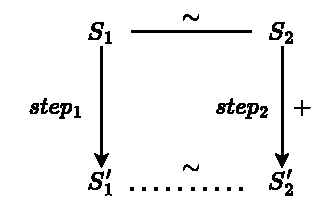
\includegraphics[width=1\linewidth]{figures/plusstep.pdf}
        \caption{多步模拟}
        \label{fig:plus}
    \end{subfigure}
    \begin{subfigure}[b]{0.52\textwidth}
        % \flushright
        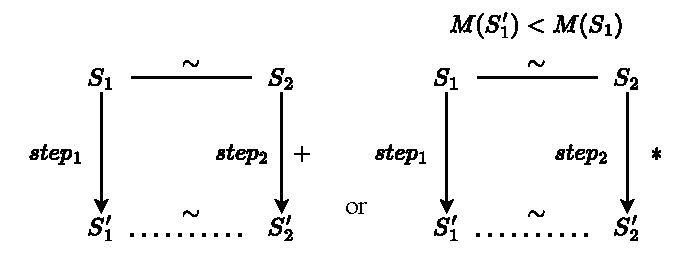
\includegraphics[width=1\linewidth]{figures/starstep2.pdf}
        \caption{星形模拟}
        \label{fig:star}
    \end{subfigure}
    \caption{不同类型的模拟图}\label{simustep}
\end{figure}

\begin{itemize}
    \item 一步模拟(Lock-Step Simulation)表示$S_2$经过一步转换到达$S'_2$状态。
        然而,对于大多数转换算法来说,一步模拟的前提要求太严格了,我们需要对其进行放宽。
    \item 多步模拟(Plus Simulation)表示$S_2$经过一步或多步转换到达$S'_2$(如图~\ref{fig:plus})。
        有时,从$S_1$到$S'_1$的转换对于状态$S_2$没有任何影响,比如删除冗余代码。
        因此,在某些情况下,多步模拟的条件也需要放松。
    \item 星形模拟(Star Simulation)表示$S_2$经过零步或一步或多步转换到达$S'_2$状态(如图~\ref{fig:star})。
        在这种条件下,可能会出现一种违反语义保存性质的情况:源程序发散,而目标程序保持在$S_2$状态,
        它们之间的状态仍然始终满足$\sim$不变式。为了防止出现这种``无限驻留''问题,我们需要
        为源程序的状态定义一个度量函数$M$,它随着源程序的执行过程严格减小。
        增添了度量函数$M$相关的限制,我们就能通过模拟保存源程序的发散行为了。
\end{itemize}

正如我们将在第~\ref{ch:verify}章中讨论的那样,CPS转换的前向模拟满足多步模拟性质,
而对于CPS到SSA的转换,我们需要使用星形模拟。根据上述模拟图性质以及
源程序和目标程序初始状态的对应关系,我们可以推导出安全程序的前向模拟。
结合目标语言的确定性,即可推导出安全程序的后向模拟。

由于语义保存性质是可传递的(Transitively Composable),
我们可以先分别证明各个编译过程的语义保存性质,然后将结果组合起来推导出整个编译过程的正确性。
例如,如果编译过程$\mathcal{T}$被分解为两个转换阶段$\mathcal{T}_1$和$\mathcal{T}_2$,
$\mathcal{T}$可以被视为它们的组合。对于一个安全的程序$P$,如果没有发生编译时错误(Compiler-Time Error),
$\mathcal{T}(P) = \mathcal{T}_2(\mathcal{T}_1(P))$。
如果我们可以验证$\mathcal{T}_1$和$\mathcal{T}_2$的正确性,那么$\mathcal{T}$也得到了验证。

\section{相关工作} \label{sec:related}

在编译器验证领域,许多工作是围绕CompCert编译器展开的,包括很多函数式语言编译器的验证工作。
例如,经验证的函数式编译器CertiCoq将Gallina(Coq语言)编译到了CompCert中使用的的Clight~\cite{belanger2019certified}。
miniML经验证的编译器也使用了CompCert框架,将其编译到了CompCert中的中间语言Cminor~\cite{dargaye2009verification}。
基于SSA的中间语言(例如LLVM IR)模块化、可移植和优化潜能大等特性引起了函数式编译器开发者的关注。
近年来,一些原本不使用SSA后端的函数式编译器已经开始转向SSA后端以获得更好的性能~\cite{farvardin2020new}。
我们的工作基于这些观察建立,是朝着构建利用SSA中间语言优势的经验证的函数式编译器迈出的第一步。

\subsection{Gallina经验证的编译器CertiCoq}

CertiCoq将Gallina编译到了C语言的子集Clight,以便与CompCert链接起来并最终编译到汇编语言,
从而获得一个完整的经过验证的编译链~\cite{belanger2019certified,zoe-oopsla2021,zoe-icfp2021}。
从CPS到Clight的编译过程及其形式化证明在Coq中实现,不过其使用的是大步操作语义而不是小步操作语义。
该编译器的目标语言不是基于SSA的,因此不能直接连接到LLVM框架,也不能利用基于SSA中间语言的优化。

\subsection{miniML经验证的编译器前端MLCompCert}

MLCompCert是Zaynah Dargaye等人设计的一个经验证的编译器前端~\cite{dargaye2009verification}。
它的源语言是ML纯函数式语言的部分,即miniML,包括了$\lambda$演算、$let$绑定、模式匹配等。
它的目标语言是CompCert编译器后端的中间语言Cminor,即一种类似于C语言的底层语言。
该编译器实现了一些经典的函数式程序编译优化,例如反柯里化(uncurrying)和统一数据结构表示等。
设计者们在Coq中对该函数式程序编译器前端进行了实现和验证。

\subsection{SML-New Jersey基于LLVM编译器后端的版本}

SML-New Jersey编译器(SML/NJ)是Standard ML的著名编译器。在最近发布的新版本中,它更改了后端,
将CPS中间语言编译到了LLVM IR~\cite{farvardin2020new}。CPS程序首先被转换为控制流图(Control-Flow Graph, CFG)中间语言,
然后再转换为LLVM IR。这是因为将CPS中间语言连接到基于SSA的编译器基础设施能够利用这些编译器提供的丰富后端优化。
但这项工作不是经过形式化验证的。
我们的工作受到了这一趋势的启发,并进一步尝试对这种连接进行形式化验证。

\subsection{CompCert支持SSA的扩展CompCertSSA}

经验证的编译器也开始试着支持基于SSA中间语言的后端了。
CompCertSSA是CompCert的一个扩展,具有一个基于SSA的中间端~\cite{compcertssa}。
它将SSA作为一种可选的优化中间语言,允许在RTL(Register Transfer Language)三地址代码和SSA中间语言之间进行转换。
虽然这使得CompCert能够实现一些基于SSA的优化~\cite{compcertssa-op,blazy-cpp2023},
但是CompCertSSA提供的优化仍然比较有限,不能与LLVM的后端优化相媲美。
不过,它提供了一个从C语言开始的经过完整验证的编译链,是开发针对SSA的经验证的函数式编译器的有力工具。

\subsection{经验证的LLVM IR: Vellvm}

Vellvm在定理证明工具Coq中定义了LLVM中间语言的抽象语法树(Abstract Syntax Tree, AST),并为LLVM IR提供了形式化语义。
早期版本的Vellvm提供了LLVM IR的操作语义~\cite{zhao2012formalizing},
而在较新版本中已迁移到了基于交互树(Interactive Tree, ITree)的语义~\cite{zakowski2021modular}。
在本文第\ref{ch:overview}章所介绍的编译链中,SSA程序首先被编译到了Vellvm AST,然后生成了最终的LLVM IR程序。

% !TEX root = ../main.tex

\chapter{数学与引用文献的标注}

\section{数学}

\subsection{数字和单位}

宏包 \pkg{siunitx} 提供了更好的数字和单位支持:
\begin{itemize}
  \item \num{12345.67890}
  \item \complexnum{1+-2i}
  \item \num{.3e45}
  \item \numproduct{1.654 x 2.34 x 3.430}
  \item \unit{kg.m.s^{-1}}
  \item \unit{\micro\meter} $\unit{\micro\meter}$
  \item \unit{\ohm} $\unit{\ohm}$
  \item \numlist{10;20}
  \item \numlist{10;20;30}
  \item \qtylist{0.13;0.67;0.80}{\milli\metre}
  \item \numrange{10}{20}
  \item \qtyrange{10}{20}{\degreeCelsius}
\end{itemize}

\subsection{数学符号和公式}

按照国标 GB/T 3102.11—1993《物理科学和技术中使用的数学符号》,
微分符号 $\dd$ 应使用直立体。除此之外,数学常数也应使用直立体:
\begin{itemize}
  \item 微分符号 $\dd$:\cs{dd}
  \item 圆周率 $\uppi$:\cs{uppi}
  \item 自然对数的底 $\ee$:\cs{ee}
  \item 虚数单位 $\ii$, $\jj$:\cs{ii} \cs{jj}
\end{itemize}

公式应另起一行居中排版。公式后应注明编号,按章顺序编排,编号右端对齐。
\begin{equation}
  \ee^{\ii\uppi} + 1 = 0,
\end{equation}
\begin{equation}
  \frac{\dd^2 u}{\dd t^2} = \int f(x) \dd x.
\end{equation}

公式末尾是需要添加标点符号的,至于用逗号还是句号,取决于公式下面一句是接着公式说的,还是另起一句。
\begin{equation}
  \frac{2h}{\pi}\int_{0}^{\infty}\frac{\sin\left( \omega\delta \right)}{\omega}
  \cos\left( \omega x \right) \dd\omega = 
  \begin{cases}
    h, & \left| x \right| < \delta, \\
    \frac{h}{2}, & x = \pm \delta, \\
    0, & \left| x \right| > \delta.
  \end{cases}
\end{equation}
公式较长时最好在等号“$=$”处转行。
\begin{align}
    & I (X_3; X_4) - I (X_3; X_4 \mid X_1) - I (X_3; X_4 \mid X_2) \nonumber \\
  = & [I (X_3; X_4) - I (X_3; X_4 \mid X_1)] - I (X_3; X_4 \mid \tilde{X}_2) \\
  = & I (X_1; X_3; X_4) - I (X_3; X_4 \mid \tilde{X}_2).
\end{align}

如果在等号处转行难以实现,也可在 $+$、$-$、$\times$、$\div$ 运算符号处转行,转行
时运算符号仅书写于转行式前,不重复书写。
\begin{multline}
  \frac{1}{2} \Delta (f_{ij} f^{ij}) =
    2 \left(\sum_{i<j} \chi_{ij}(\sigma_{i} - \sigma_{j})^{2}
    + f^{ij} \nabla_{j} \nabla_{i} (\Delta f) \right. \\
  \left. + \nabla_{k} f_{ij} \nabla^{k} f^{ij} +
    f^{ij} f^{k} \left[2\nabla_{i}R_{jk}
    - \nabla_{k} R_{ij} \right] \vphantom{\sum_{i<j}} \right).
\end{multline}

\subsection{定理环境}

示例文件中使用 \pkg{ntheorem} 宏包配置了定理、引理和证明等环境。用户也可以使用
\pkg{amsthm} 宏包。

这里举一个“定理”和“证明”的例子。
\begin{theorem}[留数定理]
\label{thm:res}
  假设 $U$ 是复平面上的一个单连通开子集,$a_1, \ldots, a_n$ 是复平面上有限个点,
  $f$ 是定义在 $U \backslash \{a_1, \ldots, a_n\}$ 上的全纯函数,如果 $\gamma$
  是一条把 $a_1, \ldots, a_n$ 包围起来的可求长曲线,但不经过任何一个 $a_k$,并且
  其起点与终点重合,那么:

  \begin{equation}
    \label{eq:res}
    \oint\limits_\gamma f(z)\, \dd z = 2\uppi \ii \sum_{k=1}^n \operatorname{I}(\gamma, a_k) \operatorname{Res}(f, a_k).
  \end{equation}

  如果 $\gamma$ 是若尔当曲线,那么 $\operatorname{I}(\gamma, a_k) = 1$,因此:

  \begin{equation}
    \label{eq:resthm}
    \oint\limits_\gamma f(z)\, \dd z = 2\uppi \ii \sum_{k=1}^n \operatorname{Res}(f, a_k).
  \end{equation}

  在这里,$\operatorname{Res}(f, a_k)$ 表示 $f$ 在点 $a_k$ 的留数,
  $\operatorname{I}(\gamma, a_k)$ 表示 $\gamma$ 关于点 $a_k$ 的卷绕数。卷绕数是
  一个整数,它描述了曲线 $\gamma$ 绕过点 $a_k$ 的次数。如果 $\gamma$ 依逆时针方
  向绕着 $a_k$ 移动,卷绕数就是一个正数,如果 $\gamma$ 根本不绕过 $a_k$,卷绕数
  就是零。

  定理~\ref{thm:res} 的证明。

  \begin{proof}
    首先,由……

    其次,……

    所以……
  \end{proof}
\end{theorem}

\section{引用文献的标注}

按照教务处的要求,参考文献外观应符合国标 GB/T 7714 的要求。模版使用 \BibLaTeX{}
配合 \pkg{biblatex-gb7714-2015} 样式包%
\footnote{\url{https://www.ctan.org/pkg/biblatex-gb7714-2015}}%
控制参考文献的输出样式,后端采用 \pkg{biber} 管理文献。

请注意 \pkg{biblatex-gb7714-2015} 宏包 2016 年 9 月才加入 CTAN,如果你使用的
\TeX{} 系统版本较旧,可能没有包含 \pkg{biblatex-gb7714-2015} 宏包,需要手动安装。
\BibLaTeX{} 与 \pkg{biblatex-gb7714-2015} 目前在活跃地更新,为避免一些兼容性问
题,推荐使用较新的版本。

正文中引用参考文献时,使用 \verb|\cite{key1,key2,key3...}| 可以产生“上标引用的参
考文献”,如 \cite{Yu2001,Cheng1999,LSC1957}。使用
\verb|\parencite{key1,key2,key3...}| 则可以产生水平引用的参考文献,例如
\parencite{Li1999,Jiang1989,Hopkinson1999}。请看下面的例子,将会穿插使用水平的和
上标的参考文献:普通图书\parencite{Yu2001,Jiang1998},论文集、会议录
\cite{CSTAM1990},科技报告\parencite{WHO1970},学位论文\cite{Zhang1998},专利文
献\parencite{Jiang1989,HBLZ2001},专著中析出的文献\cite{Cheng1999,GBT2659},期刊
中析出的文献\parencite{Li1999,Li2000},报纸中析出的文献\cite{Ding2000}, 电子文献
\parencite{Jiang1999,Christine1998,Xiao2001}。

可以使用 \verb|\nocite{key1,key2,key3...}| 将参考文献条目加入到文献表中但不在正
文中引用。使用 \verb|\nocite{*}| 可以将参考文献数据库中的所有条目加入到文献表
中。
\nocite{Yang1999,Schinstock2000,Wen1990,GBT16159}

% % !TeX root = ../main.tex

\chapter{浮动体}

\section{插图}

插图功能是利用 \TeX{} 的特定编译程序提供的机制实现的,不同的编译程序支持不同的图
形方式。有的同学可能听说“\LaTeX{} 只支持 EPS”,事实上这种说法是不准确的。\XeTeX{}
可以很方便地插入 EPS、PDF、PNG、JPEG 格式的图片。

一般图形都是处在浮动环境中。之所以称为浮动是指最终排版效果图形的位置不一定与源文
件中的位置对应,这也是刚使用 \LaTeX{} 同学可能遇到的问题。如果要强制固定浮动图形
的位置,请使用 \pkg{float} 宏包,它提供了 \texttt{[H]} 参数。

\subsection{单个图形}

图要有图题,研究生图题采用中英文对照,并置于图的编号之后,图的编号和图题应置于图
下方的居中位置。引用图应在图题右上角标出文献来源。当插图中组成部件由数字或字母等
编号表示时,可在插图下方添加图注进行说明,如图~\ref{fig:cn_100t} 所示。

\begin{figure}[!htp]
  \centering
  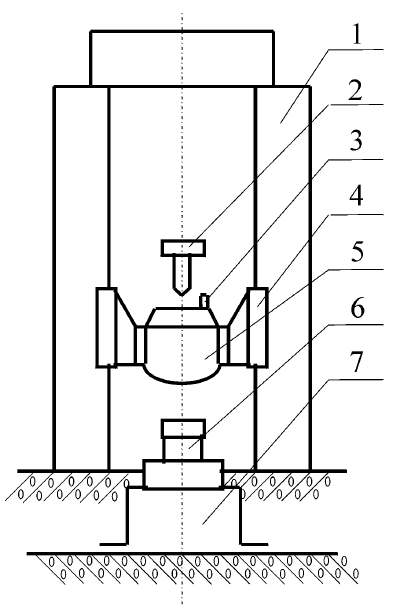
\includegraphics[width=4cm]{cn_100t.png} \\
    1.立柱 2.提升释放机构 3.标准冲击加速度计 \\
    4.导轨 5.重锤 6.被校力传感器 7.底座 \\
  \bicaption[出现在插图索引中]
    {单个图形示例\cite{He1999}。如果表格的标题很长,那么在表格索引中就会很不美观。可
      以在前面用中括号写一个简短的标题,这个标题会出现在索引中。}
    {Stay hungry, stay foolish.}
  \label{fig:cn_100t}
\end{figure}

\subsection{多个图形}

简单插入多个图形的例子如图~\ref{fig:SRR} 所示。这两个水平并列放置的子图共用一个
图形计数器,没有各自的子图题。

\begin{figure}[!htp]
  \centering
  
\includegraphics[height=2cm]{sjtu-vi-badge-blue.pdf}
  \hspace{1cm}
  
\includegraphics[height=2cm]{sjtu-vi-badge-blue.pdf}
  \bicaption{中文题图}{English caption}
  \label{fig:SRR}
\end{figure}

如果多个图形相互独立,并不共用一个图形计数器,那么用 \texttt{minipage} 或者
\texttt{parbox} 就可以,如图~\ref{fig:parallel1} 与图~\ref{fig:parallel2}。

\begin{figure}[!htp]
  \centering
  \begin{minipage}{0.48\textwidth}
    \centering
    
\includegraphics[height=1.5cm]{sjtu-vi-name-blue.pdf}
    \caption{并排第一个图}
    \label{fig:parallel1}
  \end{minipage}\hfill
  \begin{minipage}{0.48\textwidth}
    \centering
    
\includegraphics[height=1.5cm]{sjtu-vi-name-blue.pdf}
    \caption{并排第二个图}
    \label{fig:parallel2}
  \end{minipage}
\end{figure}

如果要为共用一个计数器的多个子图添加子图题,建议使用较新的 \pkg{subcaption}宏
包,不建议使用 \pkg{subfigure} 或 \pkg{subfig} 等宏包。

推荐使用 \pkg{subcaption} 宏包的 \cs{subcaptionbox} 并排子图,子图题置于子图之
下,子图号用 a)、b) 等表示。也可以使用 \pkg{subcaption} 宏包的 \cs{subcaption}
(放在 minipage中,用法同 \cs{caption})。

\pkg{subcaption} 宏包也提供了 \pkg{subfigure} 和 \pkg{subtable} 环境,如
图~\ref{fig:subfigure}。

\begin{figure}[!htp]
  \centering
  \begin{subfigure}{0.3\textwidth}
    \centering
    
\includegraphics[height=2cm]{sjtu-vi-badge-blue.pdf}
    \caption{校徽}
  \end{subfigure}
  \hspace{1cm}
  \begin{subfigure}{0.4\textwidth}
    \centering
    
\includegraphics[height=1.5cm]{sjtu-vi-name-blue.pdf}
    \caption{校名。注意这个图略矮些,subfigure 中同一行的子图在顶端对齐。}
  \end{subfigure}
  \caption{包含子图题的范例(使用 subfigure)}
  \label{fig:subfigure}
\end{figure}

搭配 \pkg{bicaption} 宏包时,可以启用 \cs{subcaptionbox} 和 \cs{subcaption} 的双
语变种 \cs{bisubcaptionbox} 和 \cs{bisubcaption},如图~\ref{fig:bisubcaptionbox}
所示。

\begin{figure}[!hbtp]
  \centering
  \bisubcaptionbox{$R_3 = 1.5\text{mm}$ 时轴承的压力分布云图}%
                  {Pressure contour of bearing when $R_3 = 1.5\text{mm}$}%
                  [6.4cm]{\includegraphics[height=3cm]{example-image-a.pdf}}
  \hspace{1cm}
  \bisubcaptionbox{$R_3 = 2.5\text{mm}$ 时轴承的压力分布云图}%
                  {Pressure contour of bearing when $R_3 = 2.5\text{mm}$}%
                  [6.4cm]{\includegraphics[height=3cm]{example-image-b.pdf}}
  \bicaption{包含子图题的范例(使用 subcaptionbox)}
            {Example with subcaptionbox}
  \label{fig:bisubcaptionbox}
\end{figure}


\section{表格}

\subsection{基本表格}

编排表格应简单明了,表达一致,明晰易懂,表文呼应、内容一致。表题置于表上,研究生
学位论文可以用中、英文两种文字居中排写,中文在上,也可以只用中文。

表格的编排建议采用国际通行的三线表\footnote{三线表,以其形式简洁、功能分明、阅读
方便而在科技论文中被推荐使用。三线表通常只有 3 条线,即顶线、底线和栏目线,没有
竖线。}。三线表可以使用 \pkg{booktabs} 提供的 \cs{toprule}、\cs{midrule} 和
\cs{bottomrule}。它们与 \pkg{longtable} 能很好的配合使用。

\begin{table}[!hpt]
  \caption[一个颇为标准的三线表]{一个颇为标准的三线表\footnotemark}
  \label{tab:firstone}
  \centering
  \begin{tabular}{@{}llr@{}} \toprule
    \multicolumn{2}{c}{Item} \\ \cmidrule(r){1-2}
    Animal & Description & Price (\$)\\ \midrule
    Gnat  & per gram  & 13.65 \\
          & each      & 0.01 \\
    Gnu   & stuffed   & 92.50 \\
    Emu   & stuffed   & 33.33 \\
    Armadillo & frozen & 8.99 \\ \bottomrule
  \end{tabular}
\end{table}
\footnotetext{这个例子来自
  \href{https://mirrors.sjtug.sjtu.edu.cn/ctan/macros/latex/contrib/booktabs/booktabs.pdf}%
  {《Publication quality tables in LaTeX》}(\pkg{booktabs} 宏包的文档)。这也是
  一个在表格中使用脚注的例子,请留意与 \pkg{threeparttable} 实现的效果有何不
  同。}

\subsection{复杂表格}

我们经常会在表格下方标注数据来源,或者对表格里面的条目进行解释。可以用
\pkg{threeparttable} 实现带有脚注的表格,如表~\ref{tab:footnote}。

\begin{table}[!htpb]
  \bicaption{一个带有脚注的表格的例子}{A Table with footnotes}
  \label{tab:footnote}
  \centering
  \begin{threeparttable}[b]
     \begin{tabular}{ccd{4}cccc}
      \toprule
      \multirow{2}*{total} & \multicolumn{2}{c}{20\tnote{a}} & \multicolumn{2}{c}{40} & \multicolumn{2}{c}{60} \\
      \cmidrule(lr){2-3}\cmidrule(lr){4-5}\cmidrule(lr){6-7}
      & www & \multicolumn{1}{c}{k} & www & k & www & k \\ % 使用说明符 d 的列会自动进入数学模式,使用 \multicolumn 对文字表头做特殊处理
      \midrule
      & $\underset{(2.12)}{4.22}$ & 120.0140\tnote{b} & 333.15 & 0.0411 & 444.99 & 0.1387 \\
      & 168.6123 & 10.86 & 255.37 & 0.0353 & 376.14 & 0.1058 \\
      & 6.761    & 0.007 & 235.37 & 0.0267 & 348.66 & 0.1010 \\
      \bottomrule
    \end{tabular}
    \begin{tablenotes}
    \item [a] the first note.
    \item [b] the second note.
    \end{tablenotes}
  \end{threeparttable}
\end{table}

如某个表需要转页接排,可以用 \pkg{longtable} 实现。接排时表题省略,表头应重复书
写,并在右上方写“续表 xx”,如表~\ref{tab:performance}。

\begin{ThreePartTable}
  \begin{TableNotes}
    \item[a] 一个脚注
    \item[b] 另一个脚注
  \end{TableNotes}
  \begin{longtable}[c]{c*{6}{r}}
    \bicaption{实验数据}{Experimental data}
    \label{tab:performance} \\
    \toprule
    测试程序 & \multicolumn{1}{c}{正常运行} & \multicolumn{1}{c}{同步}
      & \multicolumn{1}{c}{检查点} & \multicolumn{1}{c}{卷回恢复}
      & \multicolumn{1}{c}{进程迁移} & \multicolumn{1}{c}{检查点} \\
    & \multicolumn{1}{c}{时间 (s)} & \multicolumn{1}{c}{时间 (s)}
      & \multicolumn{1}{c}{时间 (s)} & \multicolumn{1}{c}{时间 (s)}
      & \multicolumn{1}{c}{时间 (s)} &  文件(KB)\\
    \midrule
    \endfirsthead
    \multicolumn{7}{l}{\textbf{续表~\thetable}} \\
    % 英语论文:\multicolumn{7}{r}{\textbf{Table~\thetable~(continued)}} \\
    \toprule
    测试程序 & \multicolumn{1}{c}{正常运行} & \multicolumn{1}{c}{同步}
      & \multicolumn{1}{c}{检查点} & \multicolumn{1}{c}{卷回恢复}
      & \multicolumn{1}{c}{进程迁移} & \multicolumn{1}{c}{检查点} \\
    & \multicolumn{1}{c}{时间 (s)} & \multicolumn{1}{c}{时间 (s)}
      & \multicolumn{1}{c}{时间 (s)} & \multicolumn{1}{c}{时间 (s)}
      & \multicolumn{1}{c}{时间 (s)}&  文件(KB)\\
    \midrule
    \endhead
    \hline
    \multicolumn{7}{r}{续下页}
    \endfoot
    \insertTableNotes
    \endlastfoot
    CG.A.2 & 23.05 & 0.002 & 0.116 & 0.035 & 0.589 & 32491 \\
    CG.A.4 & 15.06 & 0.003 & 0.067 & 0.021 & 0.351 & 18211 \\
    CG.A.8 & 13.38 & 0.004 & 0.072 & 0.023 & 0.210 & 9890 \\
    CG.B.2 & 867.45 & 0.002 & 0.864 & 0.232 & 3.256 & 228562 \\
    CG.B.4 & 501.61 & 0.003 & 0.438 & 0.136 & 2.075 & 123862 \\
    CG.B.8 & 384.65 & 0.004 & 0.457 & 0.108 & 1.235 & 63777 \\
    MG.A.2 & 112.27 & 0.002 & 0.846 & 0.237 & 3.930 & 236473 \\
    MG.A.4 & 59.84 & 0.003 & 0.442 & 0.128 & 2.070 & 123875 \\
    MG.A.8 & 31.38 & 0.003 & 0.476 & 0.114 & 1.041 & 60627 \\
    MG.B.2 & 526.28 & 0.002 & 0.821 & 0.238 & 4.176 & 236635 \\
    MG.B.4 & 280.11 & 0.003 & 0.432 & 0.130 & 1.706 & 123793 \\
    MG.B.8 & 148.29 & 0.003 & 0.442 & 0.116 & 0.893 & 60600 \\
    LU.A.2 & 2116.54 & 0.002 & 0.110 & 0.030 & 0.532 & 28754 \\
    LU.A.4 & 1102.50 & 0.002 & 0.069 & 0.017 & 0.255 & 14915 \\
    LU.A.8 & 574.47 & 0.003 & 0.067 & 0.016 & 0.192 & 8655 \\
    LU.B.2 & 9712.87 & 0.002 & 0.357 & 0.104 & 1.734 & 101975 \\
    LU.B.4 & 4757.80 & 0.003 & 0.190 & 0.056 & 0.808 & 53522 \\
    LU.B.8 & 2444.05 & 0.004 & 0.222 & 0.057 & 0.548 & 30134 \\
    EP.A.2 & 123.81 & 0.002 & 0.010 & 0.003 & 0.074 & 1834 \\
    EP.A.4 & 61.92 & 0.003 & 0.011 & 0.004 & 0.073 & 1743 \\
    EP.A.8 & 31.06 & 0.004 & 0.017 & 0.005 & 0.073 & 1661 \\
    EP.B.2 & 495.49 & 0.001 & 0.009 & 0.003 & 0.196 & 2011 \\
    EP.B.4 & 247.69 & 0.002 & 0.012 & 0.004 & 0.122 & 1663 \\
    EP.B.8 & 126.74 & 0.003 & 0.017 & 0.005 & 0.083 & 1656 \\
    SP.A.2 & 123.81 & 0.002 & 0.010 & 0.003 & 0.074 & 1854 \\
    SP.A.4 & 51.92 & 0.003 & 0.011 & 0.004 & 0.073 & 1543 \\
    SP.A.8 & 31.06 & 0.004 & 0.017 & 0.005 & 0.073 & 1671 \\
    SP.B.2 & 495.49 & 0.001 & 0.009 & 0.003 & 0.196 & 2411 \\
    SP.B.4 \tnote{a} & 247.69 & 0.002 & 0.014 & 0.006 & 0.152 & 2653 \\
    SP.B.8 \tnote{b} & 126.74 & 0.003 & 0.017 & 0.005 & 0.082 & 1755 \\
    \bottomrule
  \end{longtable}
\end{ThreePartTable}

\section{算法环境}

算法环境可以使用 \pkg{algorithms} 宏包或者较新的 \pkg{algorithm2e} 实现。
算法~\ref{algo:algorithm} 是一个使用 \pkg{algorithm2e} 的例子。关于排版算法环境
的具体方法,请阅读相关宏包的官方文档。

\begin{algorithm}[htb]
  \caption{算法示例}
  \label{algo:algorithm}
  \small
  \SetAlgoLined
  \KwData{this text}
  \KwResult{how to write algorithm with \LaTeXe }

  initialization\;
  \While{not at end of this document}{
    read current\;
    \eIf{understand}{
      go to next section\;
      current section becomes this one\;
    }{
      go back to the beginning of current section\;
    }
  }
\end{algorithm}

\section{代码环境}

我们可以在论文中插入算法,但是不建议插入大段的代码。如果确实需要插入代码,建议使
用 \pkg{listings} 宏包。

\begin{codeblock}[language=C]
#include <stdio.h>
#include <unistd.h>
#include <sys/types.h>
#include <sys/wait.h>

int main() {
  pid_t pid;

  switch ((pid = fork())) {
  case -1:
    printf("fork failed\n");
    break;
  case 0:
    /* child calls exec */
    execl("/bin/ls", "ls", "-l", (char*)0);
    printf("execl failed\n");
    break;
  default:
    /* parent uses wait to suspend execution until child finishes */
    wait((int*)0);
    printf("is completed\n");
    break;
  }

  return 0;
}
\end{codeblock}

% !TEX root = ../main.tex

\chapter{全文总结} \label{ch:summary}

\section{主要结论}

\section{研究展望}


%TC:ignore

% 参考文献
\printbibliography[heading=bibintoc]

% 附录
\appendix

% 附录中图表不加入索引
\captionsetup{list=no}

% 附录内容
% % !TEX root = ../main.tex

\chapter{Maxwell Equations}

选择二维情况,有如下的偏振矢量:
\begin{subequations}
  \begin{align}
    {\bf E} &= E_z(r, \theta) \hat{\bf z}, \\
    {\bf H} &= H_r(r, \theta) \hat{\bf r} + H_\theta(r, \theta) \hat{\bm\theta}.
  \end{align}
\end{subequations}
对上式求旋度:
\begin{subequations}
  \begin{align}
    \nabla \times {\bf E} &= \frac{1}{r} \frac{\partial E_z}{\partial\theta}
      \hat{\bf r} - \frac{\partial E_z}{\partial r} \hat{\bm\theta}, \\
    \nabla \times {\bf H} &= \left[\frac{1}{r} \frac{\partial}{\partial r}
      (r H_\theta) - \frac{1}{r} \frac{\partial H_r}{\partial\theta} \right]
      \hat{\bf z}.
  \end{align}
\end{subequations}
因为在柱坐标系下,$\overline{\overline\mu}$ 是对角的,所以 Maxwell 方程组中电场
$\bf E$ 的旋度:
\begin{subequations}
  \begin{align}
    & \nabla \times {\bf E} = \ii \omega {\bf B}, \\
    & \frac{1}{r} \frac{\partial E_z}{\partial\theta} \hat{\bf r} -
      \frac{\partial E_z}{\partial r}\hat{\bm\theta} = \ii \omega \mu_r H_r
      \hat{\bf r} + \ii \omega \mu_\theta H_\theta \hat{\bm\theta}.
  \end{align}
\end{subequations}
所以 $\bf H$ 的各个分量可以写为:
\begin{subequations}
  \begin{align}
    H_r &= \frac{1}{\ii \omega \mu_r} \frac{1}{r}
      \frac{\partial E_z}{\partial\theta}, \\
    H_\theta &= -\frac{1}{\ii \omega \mu_\theta}
      \frac{\partial E_z}{\partial r}.
  \end{align}
\end{subequations}
同样地,在柱坐标系下,$\overline{\overline\epsilon}$ 是对角的,所以 Maxwell 方程
组中磁场 $\bf H$ 的旋度:
\begin{subequations}
  \begin{align}
    & \nabla \times {\bf H} = -\ii \omega {\bf D}, \\
    & \left[\frac{1}{r} \frac{\partial}{\partial r}(r H_\theta) - \frac{1}{r}
      \frac{\partial H_r}{\partial\theta} \right] \hat{\bf z} = -\ii \omega
      {\overline{\overline\epsilon}} {\bf E} = -\ii \omega \epsilon_z E_z
      \hat{\bf z}, \\
    & \frac{1}{r} \frac{\partial}{\partial r}(r H_\theta) - \frac{1}{r}
      \frac{\partial H_r}{\partial\theta} = -\ii \omega \epsilon_z E_z.
  \end{align}
\end{subequations}
由此我们可以得到关于 $E_z$ 的波函数方程:
\begin{equation}
  \frac{1}{\mu_\theta \epsilon_z} \frac{1}{r} \frac{\partial}{\partial r}
  \left(r \frac{\partial E_z}{\partial r} \right) + \frac{1}{\mu_r \epsilon_z}
  \frac{1}{r^2} \frac{\partial^2E_z}{\partial\theta^2} +\omega^2 E_z = 0.
\end{equation}

% % !TEX root = ../main.tex

\chapter{绘制流程图}

图~\ref{fig:flow_chart} 是一张流程图示意。使用 \pkg{tikz} 环境,搭配四种预定义节
点(\verb|startstop|、\verb|process|、\verb|decision| 和 \verb|io|),可以容易地
绘制出流程图。

\begin{figure}[!htp]
  \centering
  
% 定义流程图节点
\tikzstyle{startstop} = [
  rectangle,
  rounded corners,
  minimum width=4em,
  text centered,
  inner sep=1.5ex,
  draw
]
\tikzstyle{io} = [
  trapezium,
  trapezium left angle=75,
  trapezium right angle=105,
  minimum width=4em,
  text centered,
  inner sep=1.5ex,
  draw
]
\tikzstyle{process} = [
  rectangle,
  minimum width=4em,
  text centered,
  inner sep=1.5ex,
  draw
]
\tikzstyle{decision} = [
  diamond,
  minimum width=4em,
  aspect=2,
  text centered,
  draw
]
\tikzstyle{arrow} = [-{LaTeX}]

\begin{tikzpicture}[node distance=1.5cm, every node/.style={font=\footnotesize}]
  % 设置节点
  \node[startstop] (pic) {待测图片};
  \node[io, below of=pic] (bg) {读取背景};
  \node[process, below of=bg] (pair) {匹配特征点对};
  \node[decision, below of=pair, yshift=-2ex] (threshold) {多于阈值};
  \node[decision, right of=threshold, xshift=3cm] (clear) {清晰?};
  \node[process, right of=pair, xshift=3cm] (capture) {重采};
  \node[process, below of=threshold, yshift=-2ex] (matrix_p) {透视变换矩阵};
  \node[process, right of=matrix_p, xshift=3cm] (matrix_a) {仿射变换矩阵};
  \node[process, below of=matrix_p] (reg) {图像修正};
  \node[startstop, below of=reg] (return) {配准结果};
    
  % 连接节点
  \draw[arrow] (pic) -- (bg);
  \draw[arrow] (bg) -- (pair);
  \draw[arrow] (pair) -- (threshold);

  \draw[arrow] (threshold) -- node[above] {否} (clear);

  \draw[arrow] (clear) -- node[right] {否} (capture);
  \draw[arrow] (capture) |- (pic);
  \draw[arrow] (clear) -- node[right] {是} (matrix_a);
  \draw[arrow] (matrix_a) |- (reg);

  \draw[arrow] (threshold) -- node[left] {是} (matrix_p);
  \draw[arrow] (matrix_p) -- (reg);
  \draw[arrow] (reg) -- (return);
\end{tikzpicture}

  \bicaption{绘制流程图效果}{Flow chart}
  \label{fig:flow_chart}
\end{figure}


% 结尾部分
\backmatter

% 用于盲审的论文需隐去致谢、发表论文、科研成果、简历

% 致谢
% !TEX root = ../main.tex

\begin{acknowledgements}
  感谢那位最先制作出博士学位论文 \LaTeX{} 模板的物理系同学!

  感谢 William Wang 同学对模板移植做出的贡献!

  感谢 \href{https://github.com/weijianwen}{@weijianwen} 学长开创性的工作!

  感谢 \href{https://github.com/sjtug}{@sjtug} 对 0.10 及之后版本的开发和维护工作!

  感谢所有为模板贡献过代码的\href{https://github.com/sjtug/SJTUThesis/graphs/contributors}{同学们}, 以及所有测试和使用模板的各位同学!

  感谢 \LaTeX 和 \href{https://github.com/sjtug/SJTUThesis}{SJTUThesis},帮我节省了不少时间。
\end{acknowledgements}


% 发表论文及科研成果
% 盲审论文中,发表论文及科研成果等仅以第几作者注明即可,不要出现作者或他人姓名
% !TEX root = ../main.tex

\begin{achievements}

\subsection*{学术论文}

% 明审版
\begin{bibliolist}{00}
  \item Siyu Liu and Yuting Wang. Verified Transformation of Continuation-Passing 
    Style into Static Single Assignment Form. 
    In Theoretical Aspects of Software Engineering (TASE), 2023: 20–37. 
\end{bibliolist}

% 盲审版
\begin{bibliolist*}{00}
  \item Theoretical Aspects of Software Engineering (TASE)会议(CCF-C类)文章,第一作者, 2023.
\end{bibliolist*}

\end{achievements}


% 简历
% % !TEX root = ../main.tex

\begin{resume}
  \subsection*{基本情况}
    某某,yyyy 年 mm 月生于 xxxx。

  \subsection*{教育背景}
  \begin{itemize}
    \item yyyy 年 mm 月至今,上海交通大学,博士研究生,xx 专业
    \item yyyy 年 mm 月至 yyyy 年 mm 月,上海交通大学,硕士研究生,xx 专业
    \item yyyy 年 mm 月至 yyyy 年 mm 月,上海交通大学,本科,xx 专业
  \end{itemize}

  \subsection*{研究兴趣}
    \LaTeX{} 排版

  \subsection*{联系方式}
  \begin{itemize}
    \item 地址: 上海市闵行区东川路 800 号,200240
    \item E-mail: \email{john_smith@sjtu.edu.cn}
  \end{itemize}
\end{resume}


% 学士学位论文要求在最后有一个大摘要,单独编页码
% % !TEX root = ../main.tex

\begin{digest}
  An imperial edict issued in 1896 by Emperor Guangxu, established Nanyang
  Public School in Shanghai. The normal school, school of foreign studies,
  middle school and a high school were established. Sheng Xuanhuai, the person
  responsible for proposing the idea to the emperor, became the first president
  and is regarded as the founder of the university.

  During the 1930s, the university gained a reputation of nurturing top
  engineers. After the foundation of People's Republic, some faculties were
  transferred to other universities. A significant amount of its faculty were
  sent in 1956, by the national government, to Xi'an to help build up Xi'an Jiao
  Tong University in western China. Afterwards, the school was officially
  renamed Shanghai Jiao Tong University.

  Since the reform and opening up policy in China, SJTU has taken the lead in
  management reform of institutions for higher education, regaining its vigor
  and vitality with an unprecedented momentum of growth. SJTU includes five
  beautiful campuses, Xuhui, Minhang, Luwan Qibao, and Fahua, taking up an area
  of about \qty{3225833}{\square\metre}. A number of disciplines have been
  advancing towards the top echelon internationally, and a batch of burgeoning
  branches of learning have taken an important position domestically.

  Today SJTU has 31 schools (departments), 63 undergraduate programs, 250
  masters-degree programs, 203 Ph.D. programs, 28 post-doctorate programs, and
  11 state key laboratories and national engineering research centers.

  SJTU boasts a large number of famous scientists and professors, including 35
  academics of the Academy of Sciences and Academy of Engineering, 95 accredited
  professors and chair professors of the ``Cheung Kong Scholars Program'' and
  more than \num{2000} professors and associate professors.

  Its total enrollment of students amounts to \num{35929}, of which \num{1564}
  are international students. There are \num{16802} undergraduates, and
  \num{17563} masters and Ph.D. candidates. After more than a century of
  operation, Jiao Tong University has inherited the old tradition of ``high
  starting points, solid foundation, strict requirements and extensive
  practice.'' Students from SJTU have won top prizes in various competitions,
  including ACM International Collegiate Programming Contest, International
  Mathematical Contest in Modeling and Electronics Design Contests. Famous
  alumni include Jiang Zemin, Lu Dingyi, Ding Guangen, Wang Daohan, Qian Xuesen,
  Wu Wenjun, Zou Taofen, Mao Yisheng, Cai Er, Huang Yanpei, Shao Lizi, Wang An
  and many more. More than 200 of the academics of the Chinese Academy of
  Sciences and Chinese Academy of Engineering are alumni of Jiao Tong
  University.
\end{digest}


%TC:endignore

\end{document}
